\section{The case $[2 \times 3, 6]_4$}
\begin{lemma}
  Let $p = (p_3, p_4, p_5, \dots, p_n)$ be a given sequence satisfying equation \ref{eq:valence:4} as well as $p_4 \leq 3$, $p_5 \leq 3$ and $3 \mid 2 \sum_{k=3}^{n} p_k - 4$. Then there exists $r \in \nats$ for which $p + r [2 \times 3, 6]_3$ is $4$-realizable.

  All the requirements in the statement will help utilizing Eberhards \ref{thm:eberhard:3}. The conditions $p_4 \leq 3$, $p_5 \leq 3$ deal with different sign of curvatures when having valence $3$ and $4$ (note that quadrangles and pentagons have positive curvature in the case of $3$-valence but zero or negative curvature in the other case), while the condition $p_4 \leq 3$, $p_5 \leq 3$ is necessary to keep the number of triangles natural. 
  \begin{proof}
    One can restate \ref{eq:valence:4} to a form looking more like \ref{eq:valence:3}:
    \begin{align*}
      & \sum_{k=3}^n \left( 4 - k \right) p_k = 8 \\
      \implies & \sum_{k=3}^n \left( 6 - k \right) p_k - \left(2 \sum_{k=3}^n  p_k - 4 \right) = 12
    \end{align*}
    Let $r_3 := (2 \sum_{k=3}^{n} p_k - 4)/3$. From
    \begin{align*}
      3 r_3 &= 2 \sum_{k=3}^{n} p_k - 4 =  2 p_3 + 2 p_4 + 2 p_5 + 2 \sum_{k=6}^{n} p_k - 4\\
      \implies 3 r_3 - 2 p_3 &= 2 p_4 + 2 p_5 - 4 + 2 \sum_{k=6}^{n} p_k \leq 8 + 2 \sum_{k=6}^{n} p_k \leq 8 + \sum_{k=4}^{n} (k - 4) p_k = p_3
    \end{align*}
    follows, that $p_3' := p_3 - r_3 \geq 0$ and setting $p_k' := p_k$, $(k \geq 4)$ the resulting sequence $p'$ suffices \ref{eq:valence:3}. Using \ref{thm:eberhard:3} one get a $3$-realization $P'$ of $p'$. Inserting in $P'$ an hexagon for every edge and four triangles for every vertex as seen in the following figure one can construct a $4$-realization of some sequence $p''$.
    \begin{figure}[htpp]
      \centering
      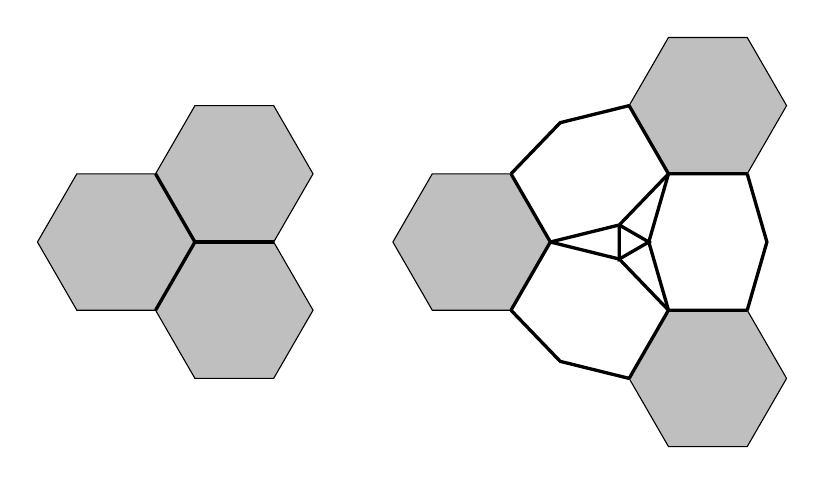
\begin{tikzpicture}
        \matrix (m) [ column sep=1cm] {
          \begin{scope}[xscale=1.0, yscale=0.866]
            \filldraw[fill=gray!50!white] (0, 1) -- ++(0.5, -1) -- ++(1, 0) -- ++(0.5, 1) -- ++(-0.5, 1) -- ++(-1, 0) -- ++(-0.5, -1);
            \filldraw[fill=gray!50!white] (1.5, 0) -- ++(0.5, -1) -- ++(1, 0) -- ++(0.5, 1) -- ++(-0.5, 1) -- ++(-1, 0) -- ++(-0.5, -1);
            \filldraw[fill=gray!50!white] (1.5, 2) -- ++(0.5, -1) -- ++(1, 0) -- ++(0.5, 1) -- ++(-0.5, 1) -- ++(-1, 0) -- ++(-0.5, -1);
            \draw[very thick] (1.5, 0) -- ++(0.5, 1) -- ++(-0.5, 1);
            \draw[very thick] (2, 1) -- ++(1, 0);
          \end{scope}
          &
          \begin{scope}[xscale=1.0, yscale=0.866] 
            \filldraw[fill=gray!50!white] (-1.5, 1) -- ++(0.5, -1) -- ++(1, 0) -- ++(0.5, 1) -- ++(-0.5, 1) -- ++(-1, 0) -- ++(-0.5, -1);
            \filldraw[fill=gray!50!white] (1.5, -1) -- ++(0.5, -1) -- ++(1, 0) -- ++(0.5, 1) -- ++(-0.5, 1) -- ++(-1, 0) -- ++(-0.5, -1);
            \filldraw[fill=gray!50!white] (1.5, 3) -- ++(0.5, -1) -- ++(1, 0) -- ++(0.5, 1) -- ++(-0.5, 1) -- ++(-1, 0) -- ++(-0.5, -1);
            \draw[very thick] (0, 0) -- ++(0.5, 1) -- ++(-0.5, 1);
            \draw[very thick] (1.5, -1) -- ++(0.5, 1) -- ++(1, 0);
            \draw[very thick] (1.5, 3) -- ++(0.5, -1) -- ++(1, 0);

            \draw[very thick] (0.5, 1) -- (1.375, 1.25) -- (2, 2);
            \draw[very thick] (0.5, 1) -- (1.375, 0.75) -- (2, 0);
            \draw[very thick] (2, 0) -- (1.75, 1) -- (2, 2);
            \draw[very thick] (1.375, 1.25) -- (1.375, 0.75) -- (1.75, 1) -- (1.375, 1.25);
            \draw[very thick] (0, 2) -- (0.625, 2.75) -- (1.5, 3);
            \draw[very thick] (0, 0) -- (0.625, -0.75) -- (1.5, -1);
            \draw[very thick] (3, 0) -- (3.25, 1) -- (3, 2);

          \end{scope};
          \\
        };
      \end{tikzpicture}
    \end{figure}
    $p''$ coincides with $p$ for every entry but $3$ and $6$. They both comply with \ref{eq:valence:4}, therefore
    \begin{align*}
      & \sum_{k=3}^n \left( 4 - k \right) p''_k  - \sum_{k=3}^n \left( 4 - k \right) p_k = 0 \\
      \implies & 2(p''_3 - p_3) = p''_6 - p_6
    \end{align*}
    and $p'' = p + (p''_6 - p_6)[2 \times 3, 6]_4$ is $4$-realizable, which finishes the proof.
  \end{proof}
\end{lemma}

\begin{lemma}
  Let $p = (p_3, p_4, p_5, \dots, p_n)$ and $q = (q_3, q_4, q_5, \dots, q_m)$ be two sequence which can be realized up to a scalar multiple of $[2 \times 3, 6]_4$, then the sequence $p + q - [8 \times 3]_4$ is $4$-realizable, also up to some scalar factor.
  \begin{proof}
    Let $P$ and $Q$ by the $4$-realizations of $p$ and $q$. By extruding every face of both realizations as seen below, adding multiple hexagons and triangles around each one, a much larger complex is build.
    \begin{figure}[htpp]
      \centering
      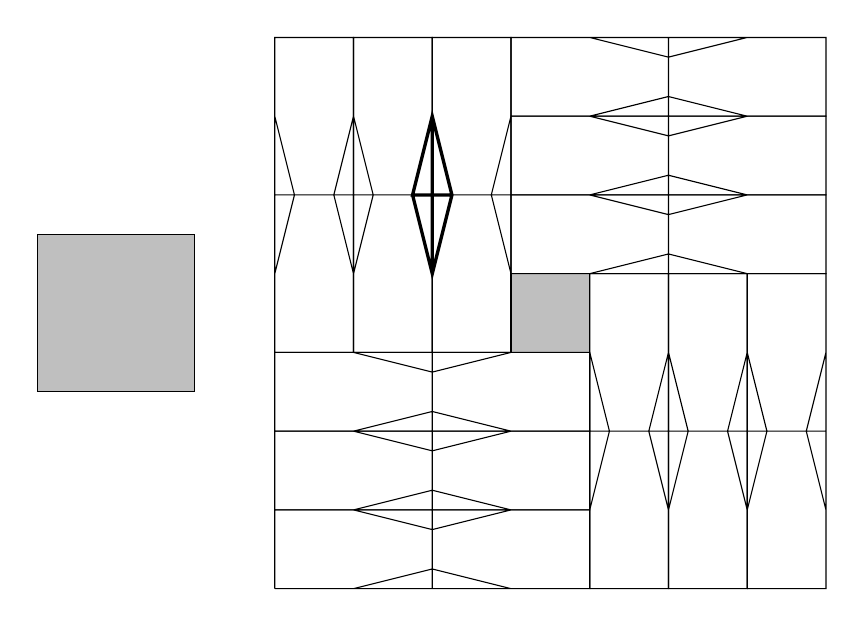
\begin{tikzpicture}
        \matrix (m) [ column sep=1cm] {
          \begin{scope}
            \filldraw[fill=gray!50!white] (-1, -1) -- (-1, 1) -- (1, 1) -- (1, -1) -- (-1, -1);
            %\draw[very thick] (-1, -1) -- (-1, 1) -- (1, 1) -- (1, -1) -- (-1, -1);
          \end{scope}
          &
          \begin{scope}[scale=0.5] 
            \filldraw[fill=gray!50!white] (-1, -1) -- (-1, 1) -- (1, 1) -- (1, -1) -- (-1, -1);
            %\draw[very thick] (-1, -1) -- (-1, 1) -- (1, 1) -- (1, -1) -- (-1, -1);
            -2) ++(-1, 0) -- ++(-0.5, 2);
            \draw (-7, -1) -- ++(2, 0) -- ++(0, 8) -- ++(-2, 0) -- ++(0, -8) ++(0, 2) -- ++(0.5, 2) ++(1, 0) -- ++(0.5, -2) ++(0, 4) -- ++(-0.5, -2) ++(-1, 0) -- ++(-0.5, 2) ++(0, -2) -- ++(2, 0);
            \draw (-5, -1) -- ++(2, 0) -- ++(0, 8) -- ++(-2, 0) -- ++(0, -8) ++(0, 2) -- ++(0.5, 2) ++(1, 0) -- ++(0.5, -2) ++(0, 4) -- ++(-0.5, -2) ++(-1, 0) -- ++(-0.5, 2) ++(0, -2) -- ++(2, 0);
            \draw (-3, -1) -- ++(2, 0) -- ++(0, 8) -- ++(-2, 0) -- ++(0, -8) ++(0, 2) -- ++(0.5, 2) ++(1, 0) -- ++(0.5, -2) ++(0, 4) -- ++(-0.5, -2) ++(-1, 0) -- ++(-0.5, 2) ++(0, -2) -- ++(2, 0);

            \draw (-7, -3) -- ++(0, 2) -- ++(8, 0) -- ++(0, -2) -- ++(-8, 0) ++(2,0) -- ++(2, 0.5) ++(0, 1) -- ++(-2, 0.5) ++(4, 0) -- ++(-2, -0.5) ++(0, -1) -- ++(2, -0.5) ++(-2, 0) -- ++(0, 2);
            \draw (-7, -5) -- ++(0, 2) -- ++(8, 0) -- ++(0, -2) -- ++(-8, 0) ++(2,0) -- ++(2, 0.5) ++(0, 1) -- ++(-2, 0.5) ++(4, 0) -- ++(-2, -0.5) ++(0, -1) -- ++(2, -0.5) ++(-2, 0) -- ++(0, 2);
            \draw (-7, -7) -- ++(0, 2) -- ++(8, 0) -- ++(0, -2) -- ++(-8, 0) ++(2,0) -- ++(2, 0.5) ++(0, 1) -- ++(-2, 0.5) ++(4, 0) -- ++(-2, -0.5) ++(0, -1) -- ++(2, -0.5) ++(-2, 0) -- ++(0, 2);

            \draw (-1, 1) -- ++(0, 2) -- ++(8, 0) -- ++(0, -2) -- ++(-8, 0) ++(2,0) -- ++(2, 0.5) ++(0, 1) -- ++(-2, 0.5) ++(4, 0) -- ++(-2, -0.5) ++(0, -1) -- ++(2, -0.5) ++(-2, 0) -- ++(0, 2);
            \draw (-1, 3) -- ++(0, 2) -- ++(8, 0) -- ++(0, -2) -- ++(-8, 0) ++(2,0) -- ++(2, 0.5) ++(0, 1) -- ++(-2, 0.5) ++(4, 0) -- ++(-2, -0.5) ++(0, -1) -- ++(2, -0.5) ++(-2, 0) -- ++(0, 2);
            \draw (-1, 5) -- ++(0, 2) -- ++(8, 0) -- ++(0, -2) -- ++(-8, 0) ++(2,0) -- ++(2, 0.5) ++(0, 1) -- ++(-2, 0.5) ++(4, 0) -- ++(-2, -0.5) ++(0, -1) -- ++(2, -0.5) ++(-2, 0) -- ++(0, 2);

            \draw (1, -7) -- ++(2, 0) -- ++(0, 8) -- ++(-2, 0) -- ++(0, -8) ++(0, 2) -- ++(0.5, 2) ++(1, 0) -- ++(0.5, -2) ++(0, 4) -- ++(-0.5, -2) ++(-1, 0) -- ++(-0.5, 2) ++(0, -2) -- ++(2, 0);
            \draw (3, -7) -- ++(2, 0) -- ++(0, 8) -- ++(-2, 0) -- ++(0, -8) ++(0, 2) -- ++(0.5, 2) ++(1, 0) -- ++(0.5, -2) ++(0, 4) -- ++(-0.5, -2) ++(-1, 0) -- ++(-0.5, 2) ++(0, -2) -- ++(2, 0);
            \draw (5, -7) -- ++(2, 0) -- ++(0, 8) -- ++(-2, 0) -- ++(0, -8) ++(0, 2) -- ++(0.5, 2) ++(1, 0) -- ++(0.5, -2) ++(0, 4) -- ++(-0.5, -2) ++(-1, 0) -- ++(-0.5, 2) ++(0, -2) -- ++(2, 0);
            \draw[very thick] (-3.5, 3) -- ++(0.5, -2) -- ++(0.5, 2) -- ++(-0.5, 2) -- ++(-0.5, -2) -- ++(1, 0) ++(-0.5, -2) -- ++(0, 4);
          \end{scope};
          \\
        };
      \end{tikzpicture}
    \end{figure}
    Each of the realizations $P$ and $Q$ has at least one of the diamond shaped construct consisting of four triangles which is marked by thick lines in the figure. By removing these four triangles on both of them one can ``glue'' the resulting quadrangles together, the established polyhedron has the desired number of faces.
  \end{proof}
\end{lemma}

\begin{lemma}
  There exists no 4-valent connected planar graph without monogons or digons where each but one face is a $k$-gon for some $k \in \nats$, $3 | k$. The single face with a number of edges not divisible by $3$ is called the exceptional face.
  \begin{proof} The proof is made by contradiction. Let $G$ be a graph with the mentioned properties. The proof shows that $G$ by reducing the number of edges $G$ can be reduced to another graph which does not meet the requirements. The first thing to notice is that one can assume the number of edges of the exceptional face to be four or five. In fact, by changing two edges it is possible to ``cut out'' a square or a pentagon from larger exceptional faces.
    In the figures below let $B$ be the exceptional face with $b$ edges. Under the transformation $B$ is reduced to a square or a pentagon, depending on whether $b \equiv 1 (\operatorname{mod} 3)$ or $b \equiv 2 (\operatorname{mod} 3)$. In the first case $E$ has $b - 4$ edges, in the second $b-5$. Therefore, in either case $E$ is not an exceptional face, its number of edges is divisible by $3$. If $A$ and $C$ are different faces the resulting graph is connected. As $A$ and $C$ have a number of edges which is divisible by $3$, so has the new face $D$. It remains the case that $A$ is the same face as $C$. Then the free space labeled with $D$ is separated by two cycles of length $d$ (denoting the length of ``left'' cycle) and $d'$ (denoting the length of ``right'' cycle). If $d$ is divisible by $3$ then the left component has exactly one exceptional face and has fewer edges then the original one. If $d$ is not divisible by $3$, then neither is $d'$, as their sum matches the sum of the number of edges of $A$ and $C$, thus the right component has exactly one exceptional face (the cycle labeled with $d'$) and fewer faces then $G$.
    \begin{figure}[htpp]
      \centering
      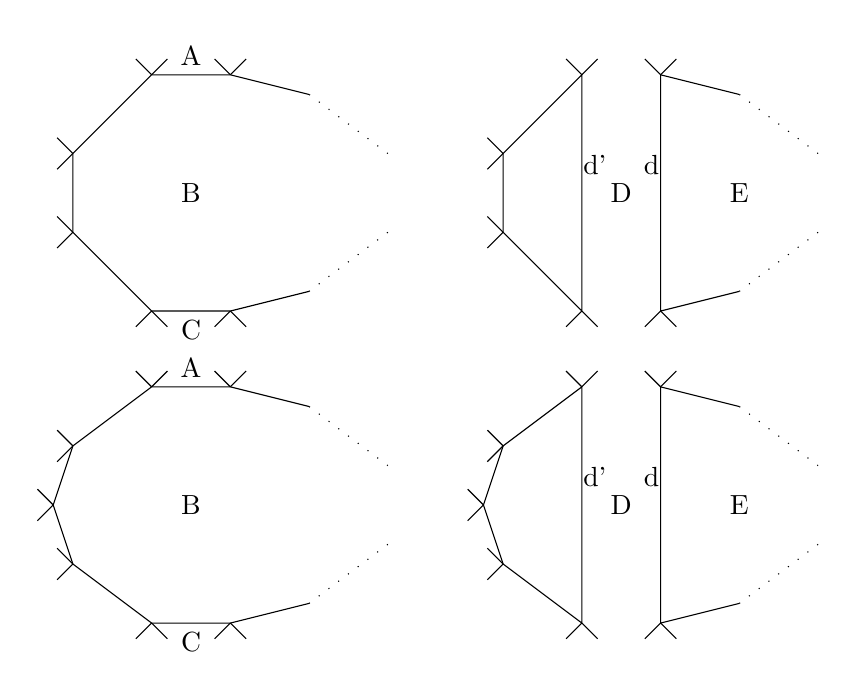
\begin{tikzpicture}
        \matrix (m) [ column sep=1cm] {
          \begin{scope}
            \draw[loosely dotted] (4, 1) -- (3, 0.25);
            \draw (3, 0.25) -- (2, 0) -- (1, 0) -- (0, 1) -- (0, 2) -- (1, 3) -- (2, 3) -- (3, 2.75);
            \draw[loosely dotted] (3, 2.75) -- (4, 2);
            \draw (2, 0) -- ++(-0.2, -0.2)  ++(0.2, 0.2) -- ++(0.2, -0.2);
            \draw (1, 0) -- ++(-0.2, -0.2)  ++(0.2, 0.2) -- ++(0.2, -0.2);
            \draw (0, 2) -- ++(-0.2, -0.2)  ++(0.2, 0.2) -- ++(-0.2, 0.2);
            \draw (0, 1) -- ++(-0.2, -0.2)  ++(0.2, 0.2) -- ++(-0.2, 0.2);
            \draw (1, 3) -- ++(0.2, 0.2)  ++(-0.2, -0.2) -- ++(-0.2, 0.2);
            \draw (2, 3) -- ++(0.2, 0.2)  ++(-0.2, -0.2) -- ++(-0.2, 0.2);
            \node [above] at (1.5, 3) {A};
            \node at (1.5, 1.5) {B};
            \node [below] at (1.5, 0) {C};
          \end{scope}
          &
          \begin{scope}
            \draw[loosely dotted] (4, 1) -- (3, 0.25);
            \draw (3, 0.25) -- (2, 0) -- (2, 3) node [midway, above=10pt, left=-3pt] {d} -- (3, 2.75);
            \draw (1, 0) -- (0, 1) -- (0, 2) -- (1, 3) -- (1, 0) node [midway, above=10pt, right=-3pt] {d'};
            \draw[loosely dotted] (3, 2.75) -- (4, 2);
            \draw (2, 0) -- ++(-0.2, -0.2)  ++(0.2, 0.2) -- ++(0.2, -0.2);
            \draw (1, 0) -- ++(-0.2, -0.2)  ++(0.2, 0.2) -- ++(0.2, -0.2);
            \draw (0, 2) -- ++(-0.2, -0.2)  ++(0.2, 0.2) -- ++(-0.2, 0.2);
            \draw (0, 1) -- ++(-0.2, -0.2)  ++(0.2, 0.2) -- ++(-0.2, 0.2);
            \draw (1, 3) -- ++(0.2, 0.2)  ++(-0.2, -0.2) -- ++(-0.2, 0.2);
            \draw (2, 3) -- ++(0.2, 0.2)  ++(-0.2, -0.2) -- ++(-0.2, 0.2);
            \node at (1.5, 1.5) {D};
            \node at (3, 1.5) {E};
          \end{scope}
          \\
          \begin{scope}
            \draw[loosely dotted] (4, 1) -- (3, 0.25);
            \draw (3, 0.25) -- (2, 0) -- (1, 0) -- (0, 0.75) -- (-0.25, 1.5) -- (0, 2.25) -- (1, 3) -- (2, 3) -- (3, 2.75);
            \draw[loosely dotted] (3, 2.75) -- (4, 2);
            \draw (2, 0) -- ++(-0.2, -0.2)  ++(0.2, 0.2) -- ++(0.2, -0.2);
            \draw (1, 0) -- ++(-0.2, -0.2)  ++(0.2, 0.2) -- ++(0.2, -0.2);
            \draw (0, 2.25) -- ++(-0.2, -0.2)  ++(0.2, 0.2) -- ++(-0.2, 0.2);
            \draw (-0.25, 1.5) -- ++(-0.2, -0.2)  ++(0.2, 0.2) -- ++(-0.2, 0.2);
            \draw (0, 0.75) -- ++(-0.2, -0.2)  ++(0.2, 0.2) -- ++(-0.2, 0.2);
            \draw (1, 3) -- ++(0.2, 0.2)  ++(-0.2, -0.2) -- ++(-0.2, 0.2);
            \draw (2, 3) -- ++(0.2, 0.2)  ++(-0.2, -0.2) -- ++(-0.2, 0.2);
            \node [above] at (1.5, 3) {A};
            \node at (1.5, 1.5) {B};
            \node [below] at (1.5, 0) {C};
          \end{scope}
          &
          \begin{scope}
            \draw[loosely dotted] (4, 1) -- (3, 0.25);
            \draw (3, 0.25) -- (2, 0) -- (2, 3) node [midway, above=10pt, left=-3pt] {d} -- (3, 2.75);
            \draw (1, 0) -- (0, 0.75) -- (-0.25, 1.5) -- (0, 2.25) -- (1, 3) -- (1, 0) node [midway, above=10pt, right=-3pt] {d'};
            \draw[loosely dotted] (3, 2.75) -- (4, 2);
            \draw (2, 0) -- ++(-0.2, -0.2)  ++(0.2, 0.2) -- ++(0.2, -0.2);
-- (-3, -3) -- (-3.125, -2.25)            \draw (1, 0) -- ++(-0.2, -0.2)  ++(0.2, 0.2) -- ++(0.2, -0.2);
            \draw (0, 2.25) -- ++(-0.2, -0.2)  ++(0.2, 0.2) -- ++(-0.2, 0.2);
            \draw (-0.25, 1.5) -- ++(-0.2, -0.2)  ++(0.2, 0.2) -- ++(-0.2, 0.2);
            \draw (0, 0.75) -- ++(-0.2, -0.2)  ++(0.2, 0.2) -- ++(-0.2, 0.2);
            \draw (1, 3) -- ++(0.2, 0.2)  ++(-0.2, -0.2) -- ++(-0.2, 0.2);
            \draw (2, 3) -- ++(0.2, 0.2)  ++(-0.2, -0.2) -- ++(-0.2, 0.2);
            \node at (1.5, 1.5) {D};
            \node at (3, 1.5) {E};
          \end{scope}
          \\
        };
      \end{tikzpicture}
    \end{figure}

    A similar construction can be used to ``cut'' out a triangle from a larger non exceptional face ($B$). 
    
    \begin{figure}[htpp]
      \centering
      \begin{tikzpicture}
        \matrix (m) [ column sep=1cm] {
          \begin{scope}
            \draw[loosely dotted] (4, 1) -- (3, 0.25);
            \draw (3, 0.25) -- (2, 0) -- (1, 0) -- (0, 1.5) -- (1, 3) -- (2, 3) -- (3, 2.75);
            \draw[loosely dotted] (3, 2.75) -- (4, 2);
            \draw (2, 0) -- ++(-0.2, -0.2)  ++(0.2, 0.2) -- ++(0.2, -0.2);
            \draw (1, 0) -- ++(-0.2, -0.2)  ++(0.2, 0.2) -- ++(0.2, -0.2);
            \draw (0, 1.5) -- ++(-0.2, -0.2)  ++(0.2, 0.2) -- ++(-0.2, 0.2);
            \draw (1, 3) -- ++(0.2, 0.2)  ++(-0.2, -0.2) -- ++(-0.2, 0.2);
            \draw (2, 3) -- ++(0.2, 0.2)  ++(-0.2, -0.2) -- ++(-0.2, 0.2);
            \node [above] at (1.5, 3) {A};
            \node at (1.5, 1.5) {B};
            \node [below] at (1.5, 0) {C};
          \end{scope}
          &
          \begin{scope}
            \draw[loosely dotted] (4, 1) -- (3, 0.25);
            \draw (3, 0.25) -- (2, 0) -- (2, 3) node [midway, above=10pt, left=-3pt] {d} -- (3, 2.75);
            \draw (1, 0) -- (0, 1.5) -- (1, 3) -- (1, 0) node [midway, above=10pt, right=-3pt] {d'};
            \draw[loosely dotted] (3, 2.75) -- (4, 2);
            \draw (2, 0) -- ++(-0.2, -0.2)  ++(0.2, 0.2) -- ++(0.2, -0.2);
            \draw (1, 0) -- ++(-0.2, -0.2)  ++(0.2, 0.2) -- ++(0.2, -0.2);
            \draw (0, 1.5) -- ++(-0.2, -0.2)  ++(0.2, 0.2) -- ++(-0.2, 0.2);
            \draw (1, 3) -- ++(0.2, 0.2)  ++(-0.2, -0.2) -- ++(-0.2, 0.2);
            \draw (2, 3) -- ++(0.2, 0.2)  ++(-0.2, -0.2) -- ++(-0.2, 0.2);
            \node at (1.5, 1.5) {D};
            \node at (3, 1.5) {E};
          \end{scope}
          \\
        };
      \end{tikzpicture}
    \end{figure}
    The argument is mostly the same as in the previos case. $E$ has three less edges the $B$, the number of whose are divisible by $3$. There is also a differentiation to be made whether $A$ and $C$ denote the same face. If not, then the resulting graph is connected and has a triangle. If they are the same the graph separates and one of both sides has exactly one exceptional face and has fewer edges then $G$.

    This step will be used for the up to eight or ten faces which share at least one vertex with the exceptional face (eight if it is a square, ten if it is a pentagon). One can therefore assume that the exceptional face is surrounded by triangles, else one could try the above step to ``cut out'' a triangle, resulting in fewer edges or in a triangle at the desired position. But the resulting graph is isomorph to the skeleton of an antiprism, which has one additional exceptional face. The steps taken did not introduce new exceptional faces, a contradiction.
    \begin{figure}[htpp]
      \centering
      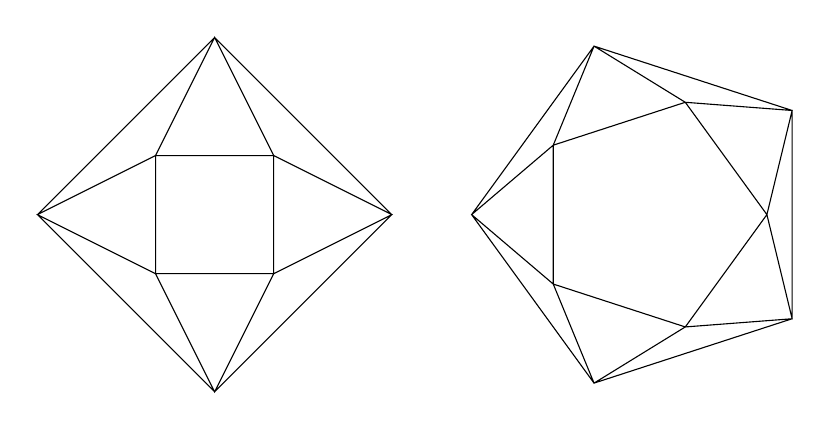
\begin{tikzpicture}
        \matrix (m) [ column sep=1cm] {
          \begin{scope}[scale=0.75]
            \draw (-1, -1) -- (-1, 1) -- (1, 1) -- (1, -1) -- (-1, -1) -- (0, -3) -- (1, -1) -- (3, 0) -- (1, 1) -- (0, 3) -- (-1, 1) -- (-3 , 0) -- (-1, -1) (0, -3) -- (3, 0) -- (0, 3) -- (-3, 0) -- (0, -3);
          \end{scope}
          &
          \begin{scope}[scale=0.75]
            \draw (0 : 2) -- (72 : 2) -- (144 : 2) -- (216 : 2) -- (288 : 2) -- (0 : 2) -- (36 : 3) -- (72 : 2) -- (108 : 3) -- (144 : 2) -- (180 : 3) -- (216 : 2) -- (252 : 3) -- (288 : 2) -- (324 : 3) -- (0 : 2) -- (36 : 3) -- (108 : 3) -- (180 : 3) -- (252 : 3) -- (324 : 3) -- (36 : 3);
          \end{scope}
          \\
        };
      \end{tikzpicture}
    \end{figure}
  \end{proof}
\end{lemma}
\begin{remark}
  The proof given is simiar to \cite{ConvexPolytopes}, where a proof for $3$-valent graphs is given. As is the case there, digons can be allowed during the argument. They do not simplify the proof here, so they were omitted.
\end{remark}
\begin{corollary}
  There is no 4-realization up to a scalar multiple of $[2 \times 3, 6]_4$ of the sequence $[1 \times k]_4$ for $3 \nmid k$.
  \begin{proof}
    Todo. Steinitz theorem.
  \end{proof}
\end{corollary}
\heartpar{kuno und susi un kuno und susi und kuno und susi und kuno}



